\documentclass[lettersize,journal]{IEEEtran}
\usepackage{amsmath,amsfonts}
\usepackage{algorithmic}
\usepackage{algorithm}
\usepackage{array}
\usepackage[caption=false,font=normalsize,labelfont=sf,textfont=sf]{subfig}
\usepackage{textcomp}
\usepackage{stfloats}
\usepackage{url}
\usepackage{verbatim}
\usepackage{graphicx}
\usepackage{cite}
\hyphenation{op-tical net-works semi-conduc-tor IEEE-Xplore}
% updated with editorial comments 8/9/2021

\usepackage{tikz}
\usetikzlibrary{shapes.geometric, arrows.meta, positioning}
\usetikzlibrary{fit, backgrounds}

\usepackage{biblatex}
\addbibresource{references.bib}

\begin{document}

\title{A Sample Article Using IEEEtran.cls\\ for IEEE Journals and Transactions}

\author{IEEE Publication Technology,~\IEEEmembership{Staff,~IEEE,}
        % <-this % stops a space
\thanks{This paper was produced by the IEEE Publication Technology Group. They are in Piscataway, NJ.}% <-this % stops a space
\thanks{Manuscript received April 19, 2021; revised August 16, 2021.}}

% The paper headers
\markboth{Journal of \LaTeX\ Class Files,~Vol.~14, No.~8, August~2021}%
{Shell \MakeLowercase{\textit{et al.}}: A Sample Article Using IEEEtran.cls for IEEE Journals}

\IEEEpubid{0000--0000/00\$00.00~\copyright~2021 IEEE}
% Remember, if you use this you must call \IEEEpubidadjcol in the second
% column for its text to clear the IEEEpubid mark.

\maketitle

\begin{abstract}
This document describes the most common article elements and how to use the IEEEtran class with \LaTeX \ to produce files that are suitable for submission to the IEEE.  IEEEtran can produce conference, journal, and technical note (correspondence) papers with a suitable choice of class options. 
\end{abstract}

\begin{IEEEkeywords}
Article submission, IEEE, IEEEtran, journal, \LaTeX, paper, template, typesetting.
\end{IEEEkeywords}

\section{Introduction}
\IEEEPARstart{B}{lah} blah blah blah this is an introduction using \LaTeX.

\begin{itemize}
    \item Orbital radar sounders are an essential tool to understand the interior of planetary bodies.
    \item There are many successful examples (MARSIS \cite{jordan_mars_2009}, SHARAD \cite{seu_sharad_2007}).
    \item Two more are on the way (RIME \cite{bruzzone_rime_2013}, REASON \cite{blankenship_radar_2024}).
    \item Existing simulators are useful to understand layered subsurfaces such as mars (ice, volcanics). \cite{gerekos_coherent_2018}
    \item For non-layered or heavily varied subsurfaces, or advanced targets or antennas finite difference based simulators are used. \cite{warren_gprmax_2016}
    \item All of these struggle at planetary scales where to discretize a subsurface you need incredible amounts of memory and huge processing times. \cite{thakur_approach_2021}
    \item Given that there are multiple planetary radars on the way to regions with likely complex heterogeneous subsurfaces \cite{schmidt_active_2011}, \cite{dicarlofelice_new_2024}, \cite{culberg_double_2022}, \cite{matteoni_evolution_2023} this means we need a new simulator which enables immediate analysis of complex subsurface returns. 
    \item Furthermore this is necessary if we ever desire to invert such areas. 
    \item Advancements in computer processing techniques enable new methods of radar simulation which capitalize on the GPU architecture and memory management techniques.
    \item We use this to make a planetary scale radar simulator we test to replicate the martian subsurface. 
    \item This means our simulator can operate efficiently and processing time has minimal dependence on operating frequency.
\end{itemize}

\section{Simulator Fundamentals}

A simulation of a full radargram is done on an individual echo by echo process where each echo corresponds to a unique source location and all of the facets and targets within that sources processing aperture. This architecture enables simulation of arbitrary non-conventional radar transects, such as drone paths, fly-bys, variable PRFs, intermittent transmitting and more. 

\subsection{Geometry Calculations}

Here we cover all of the computations associated with the geometry of an echo simulation. The software implementation is not necessarily in the same order as presented here. This is covered in \ref{sec:Software}.

We begin a simulation of an individual echo by defining our source location $\vec{s}$, facet locations $\vec{f_i}$ and target locations $\vec{t_j}$ in 3D cartesian space. We then define a local orthonormal tangent basis for each: $(\hat{n_s}, \hat{u_s}, \hat{v_s})$, $(\hat{n_{fi}}, \hat{u_{fi}}, \hat{v_{fi}})$, $(\hat{n_{tj}}, \hat{u_{tj}}, \hat{v_{tj}})$ corresponding to the source, facets and targets respectively. Note that subscript $_i$ corresponds to the facet index and $_j$ is the target index. 

$\vec{f_i}$ and $(\hat{n_{fi}}, \hat{u_{fi}}, \hat{v_{fi}})$ are generated by discretizing a arbitrary surface into a mesh of square facets with side length $l$. We take this approach from \cite{nouvel_radar_2004}. This simple process enables us to capture any scale of topography at whatever resolution is necessary to adequately model the subsurface given the simulation parameters. 

We then define the region above the surface to have a bulk relative permittivity, magnetic permability, and conductivity of $\varepsilon'_1$, $\mu_1$ and $\sigma_1$. The bulk values for the subsurface are $\varepsilon'_2$, $\mu_2$ and $\sigma_2$. Note how subscript $_1$ denotes above surface parameters and $_2$ denotes subsurface parameters. We define the propagation speeds as follows:

\begin{align}
        c_1 &= c_0\frac{1}{\sqrt{\varepsilon'_1}} \\
        c_2 &= c_0\frac{1}{\sqrt{\varepsilon'_2}}
\end{align}
Where $c_0$ is the speed of light in a vacuum. 

We can then define the incident raypaths $\vec{I_{i}}$ corresponding to the path of propagation from the source to every facet, where $\hat{I_{i}}$ is the normalized equivalent:
\begin{equation}
    \vec{I_{i}}=\vec{f_i}-\vec{s}
\end{equation}
Using this we compute the angle between the source normal and incident vector $\theta_{si}$:
\begin{equation}
    \theta_{si} = \arccos\left(-\hat{I_{i}}\cdot\hat{n_s}\right)
\end{equation}

To reduce computational complexity we reduce the simulation domain to the region purely within a synthetic processing aperture $\theta_A$ defined as the angle from $\hat{n_s}$ to the edge of the processing aperture cone. We evaluate if each facet is within the processing aperture:
\begin{equation}\label{eq:InAperture}
    \theta_{si} < \theta_A 
\end{equation}
For all facets which fulfill Equation \ref{eq:InAperture}, we continue the ray calculations by evaluating the incident inclination $\theta_{Ii}$ and azimuthal $\phi_{Ii}$ angles:
\begin{align}
    \theta_{Ii} &= \arccos\left(-\hat{I_{i}}\cdot\hat{n_{fi}}\right) \\
    \phi_{Ii} &= \operatorname{atan2}(\hat{I_{i}}\cdot\hat{u_i}, \hat{I_{i}}\cdot\hat{v_i})
\end{align}
We then compute the naturally refracted raypath's inclination $\theta_{Ri}$ and azimuthal $\phi_{Ri}$ angles via:
\begin{align}
    \label{eq:RSnells}
    \theta_{Ri} &= \arcsin\left(\theta_{i}\sqrt{\frac{\varepsilon'_1}{\varepsilon'_2}}\right) \\
    \phi_{Ri} &= \phi_{Ii}
\end{align}
Where Equation \ref{eq:RSnells} is a rearranged form of Snell's Law. To track total internal/external reflection we set $\theta_{Ri}$ to a very large constant to identify later.

We define $\vec{F}$ as our "forced" raypath which defines the path from each facet to each target. We calculate this as:
\begin{equation}
    \vec{F_{ij}}=\vec{t_j}-\vec{f_i}
\end{equation}
The reverse forced raypath is simply $-\vec{F_{ij}}$ representing the vector from the target to the facet. We then evaluate the angle between the target normal and the forced raypath $\Delta\theta_{t,ij}$ and the inclination and azimuthal angles relative to the facet normal $\Delta\theta_{f,ij}$, $\Delta\phi_{f,ij}$ using the following: 
\begin{align}
    \Delta\theta_{t,ij} &= \arccos\left(-\hat{F_{ij}}\cdot\hat{n_{ti}}\right) \\
    \Delta\theta_{f,ij} &= \arccos\left(-\hat{F_{ij}}\cdot\hat{n_{fi}}\right) \\
    \Delta\phi_{f,ij} &= \operatorname{atan2}(\hat{F_{ij}}\cdot\hat{u_i}, \hat{F_{ij}}\cdot\hat{v_i})
\end{align}
For the upward transmitted ray the only necessary value is the angle between $\vec{U_{ij}}$ and  $\hat{n_{fi}}$, ($\Delta\theta_{U,ij}$) which we obtain via $\Delta\theta_{f,ij}$ as for ray $i$ we know that $\Delta\theta_{f,ij}$ is identical for $-\vec{F_{ij}}$. 
\begin{equation}
    \Delta\theta_{U,ij} = \arcsin\left(\Delta\theta_{f,ij}\sqrt{\frac{\varepsilon'_2}{\varepsilon'_1}}\right)
\end{equation}

Targets can be given a custom scattering pattern through a function which maps an input ray index $i_1$ to a function of weights over output ray indices $i_2$. This enables large or complex target behavior to be embedded into a single point target. Simply put this is:
\begin{equation}
    W_{scatter}=\operatorname{scatter(i_1, i_2)}
\end{equation}
For all examples below we use the following:
\begin{equation}
    W_{scatter}=
    \begin{cases}
        1 \hspace{0.5cm} \mathrm{if} \hspace{0.5cm} i_1=i_2\\
        0\hspace{0.5cm} \mathrm{o.w.}
    \end{cases}
\end{equation}

\begin{itemize}
    \item 
    Slant range to each facet for both the reflected ($\rho_{l,i}$) and refracted raypaths ($\rho_{r,ij}$) are simple to evaluate. We compute them in the permittivity corrected form for ease of processing.
    \begin{align}
        \rho_{l,i} &= \frac{c_0}{c_1}\left\lVert\vec{I_i}\right\rVert \\
        \rho_{r,ij} &= \frac{c_0}{2c_1}\left(\left\lVert\vec{I_{i_1}}\right\rVert + \left\lVert\vec{I_{i_2}}\right\rVert \right) + \frac{c_0}{2c_2}\left(\left\lVert\vec{F_{{i_1}j}}\right\rVert + \left\lVert\vec{F_{{i_2}j}}\right\rVert\right)
    \end{align}
    \item Attenuation geometry is defined through a bulk background conductivity and then simple geometries of altered conductivity. Enabling thin layers etc etc etc. \\
    To keep processing times efficient we define heterogeneity in subsurface conductivity through accumulation of 3D geometric primitives. This leads to enormous reductions in memory requirements compared to if we had a regularly discretized subsurface. Furthermore this enables implementation of subsurface geometries which would otherwise be cumbersome to implement such as extremely thin yet highly conductivity layers. Currently only prisms are implemented, but other primitives such as triangles, ellipsoids and others are planned. To evaluate the impact of a highly conductive prism on the weight of an individual raypath we need the duration the ray is within the prism. The actual attenuation calculations are described in \ref{sec:RefrWeight}.\\
    We define the extent of a prism as $(x_{min},x_{max},y_{min},y_{max},z_{min},z_{max})$. We then evaluate the slab sections individually.\\
    First we determine if a ray is parallel to a given plane. If it is, and if the origin for that dimension is not within that dimensions slab there must be no intersection. If there is an intersection, the computation of the duration for the raypath in that dimensions slab is trivial. Note that $C$ subscript $_C$ represents an individual component of a vector, and $_k$ represents the index for a given prism.
    \begin{equation}
        \text{If } F_{C,ij} < 10^{-12}:\hspace{1mm}
        \begin{cases}
            f_{C,i} < C_{k\min} \ \text{or}\ f_{C,i} > C_{k\max} \;\Rightarrow\; \text{no hit},\\
            d_{C1ij} = -\infty,\quad d_{C2ij} = +\infty,
        \end{cases}
        \end{equation}
        
        \begin{equation}
            \text{Else:}\hspace{1mm}
            d_{C1ijk} = \frac{C_{k\min} - f_{c,i}}{F_{C,ij}}, \hspace{1mm}
            d_{C2ijk} = \frac{C_{k\max} - f_{c,i}}{F_{C,ij}},
        \end{equation}
        
        \begin{equation}
            \text{If } d_{C1ijk} > d_{C2ijk}:\hspace{2mm}
            (d_{C1ijk}, d_{C2ijk}) \leftarrow (d_{C2ijk}, d_{C1ijk}).
    \end{equation}
    \item We can then get the final duration of the ray in the attenuative prism as:
    \begin{align}
        d_{\mathrm{entry},ijk} &= \max\left(0,\max_{C \in \{x,y,z\}} d_{C1ijk}\right) \\
        d_{\mathrm{exit},ijk} &= \min\left(\left\lVert\vec{F_{ij}}\right\rVert,\min_{C \in \{x,y,z\}} d_{C2ijk}\right)\\
        d_{ijk} &= d_{\mathrm{exit},ijk}-d_{\mathrm{entry},ijk}
    \end{align}
\end{itemize}

\begin{figure}
\usetikzlibrary{calc}

\begin{tikzpicture}[
    vec/.style={black, thick, -{Latex[length=2mm]}},
    vecD/.style={black, thick, {Latex[length=2mm]}-{Latex[length=2mm]}},
    dashedvec/.style={thick, dashed, -{Latex[length=2mm]}},
    normal/.style={black, dashed, -{Latex[length=2mm]}},
    scale=1.2
]

% Interface
\pgfmathsetmacro{\wdth}{3}
\pgfmathsetmacro{\ssize}{1.5}
\pgfmathsetmacro{\dz}{0.25}
\pgfmathsetmacro{\dnx}{0.2}

\fill[gray!20] (-3,-0.5) -- (-1.8,-0.25) -- (-0.6,\dz) -- (0.6,0.0) -- (1.8,0.75) -- (3,1.0) -- (\wdth,-3) -- (-\wdth,-3) -- cycle;
\draw[thick] (-3,-0.5) -- (-1.8,-0.25) -- (-0.6,\dz) -- (0.6,0.0) -- (1.8,0.75) -- (3,1.0);

% reflected direction
% incident direction vector
\pgfmathsetmacro{\sx}{-1.5}
\pgfmathsetmacro{\sy}{2}
\pgfmathsetmacro{\ix}{0 - \sx}   % f_x - s_x
\pgfmathsetmacro{\iy}{0.125 - \sy}    % f_y - s_y

% Origin (interaction point)
\coordinate (f) at (0,0.125);
\coordinate (s) at (\sx,\sy);
\coordinate (t) at (1.5,-2.5);

% normal endpoint
\coordinate (n) at ($(f)+(\dnx,1)$);

% incident vector endpoint (relative)
\coordinate (i) at ($(f)!1!(s)$);

% normal vector
\pgfmathsetmacro{\nx}{\dnx}
\pgfmathsetmacro{\ny}{1}

% normalize normal
\pgfmathsetmacro{\nlen}{sqrt(\nx*\nx+\ny*\ny)}
\pgfmathsetmacro{\nnx}{\nx/\nlen}
\pgfmathsetmacro{\nny}{\ny/\nlen}

% dot product
\pgfmathsetmacro{\dotp}{\ix*\nnx+\iy*\nny}

% reflected vector
\pgfmathsetmacro{\rx}{0.5*(\ix-2*\dotp*\nnx)}
\pgfmathsetmacro{\ry}{0.5*(\iy-2*\dotp*\nny)}

% reflected endpoint
\coordinate (rs) at ($(f)+(\rx,\ry)$);

% incident ray
\draw[vecD] (s) -- (f) node[midway, above] {$\vec I_i$};
\fill (s) circle (\ssize pt) node[above] {$\vec{s}$};

% normal
\draw[normal] (f) -- (n) node[above] {$\hat f_{ni}$};

% reflected ray
\draw[vec] (f) -- (rs) node[right, above] {$\vec r$};
\draw[vec] (f) -- ($(f)+(-1.5,0.75)$) node[left] {$\vec{U_{ij}}$};

% Subsurf
\fill (t) circle (\ssize pt) node[right] {$\vec{t_j}$};
\draw[normal] (t) -- ($(t)+(0.5*\dnx, 1)$) node[above] {$\hat t_{nj}$};
\draw[vecD] (f) -- (t) node[midway, right] {$\vec{F_{ij}}$};
\draw[vec] (f) -- ($(t)-(1.2,-0.3)$) node[midway, left] {$\vec{R_{i}}$};

% Labels for permittivity
\node at (-2.2,0.25) {$\varepsilon_1,\mu_1,\sigma_1$};
\node at (-2.2,-2.0) {$\varepsilon_2,\mu_2,\sigma_2$};


\end{tikzpicture}
\centering
\caption{Diagram figure.}
\label{fig:diagram}
\end{figure}

\subsection{Reflected Raypath Weighting}

\begin{itemize}
    \item The 2-way losses are computed at once. 
    \item Assuming an isotropic source for now.
    \item Radar equation to find power entering facet aperture. \textit{Note how this is proportional to $n^2$}!
    \item Reradiated power based on modified facet beam pattern equation. 
    \item Reflection coefficient (refraction stored for later, but computed at the same time). 
    \item Atmospheric attenuation
    \item Surface RMS losses (just loss of energy, no moving it elsewhere). 
\end{itemize}

\label{sec:RefrWeight}
\subsection{Refracted Raypath Weighting}

\begin{itemize}
    \item In contrast to the Reflected energy, here we compute 1-way energy losses.
    \item Ray attenuation is computed during target raypath computation. This is done by updating an exponent value which is then used as the starting value for both inward and outward ray weights. 
\end{itemize}

\textbf{Inward:}
\begin{itemize}
    \item $\Delta \theta$ and $\Delta \phi$ between target and refracted rays. 
    \item Treating all targets like a facet with inputs $\Delta \theta$ and $\Delta \phi$.
    \item Refraction coefficient from before
    \item RMS losses. 
\end{itemize}

\textbf{Outward:}
\begin{itemize}
    \item Surface facet reradiation outwards based on delta between upward transmitted ray and ray to source from facet. 
    \item Transmission coefficient is the same going upwards
    \item Comp surface roughness losses
\end{itemize}

\textbf{Combination:}
\begin{itemize}
    \item Target reradiation pattern (boxcar for focusing)
    \item Radar equation over full path length
\end{itemize}

\subsection{Phasor Formulation}
\begin{itemize}
    \item Every incident ray has a phasor for the surface reflection and one for every subsurface target refraction. 
    \item Every incident ray also has a index for the range bin the surface response and every subsurface target response belongs at.
    \item Independently the surface and subsurface phasors for each target are summed at their bins. 
    \item Independently, this is convolved with the chirp to get the signal.
    \item These are summed to get the final trace. 
\end{itemize}


\section{Software Implementation}\label{sec:Software}

\begin{itemize}
    \item Each trace is computed independently and output as a separate file to be combined later by a python for figure generation and focusing.
    \item Initially compute the angle of every ray incident to the surface to the spacecraft normal. 
    \item Using this we make a mask for what is inside/outside of the processing aperture. 
    \item We crop all input facet arrays (locations, normals, incident angles) using CUDA thrust primitives. \cite{bell_thrust_2012}
    \item This enables a reduction in memory, reducing the amount of data from CPU$\rightarrow$GPU which is costly. 
    \item We compute all raypath weights in parallel on the GPU. This makes this incredibly fast and the processing time is nearly independent of the facet count. 
    \item Mention attenuation exponent
    \item Phasor and range bin computation is also done in parallel which means minimal computational cost.
    \item Using thrust primitives we "reduce by key" all of the phasors into one summed phasor trace.
    \item That is very expensive as it requires a sort of all phasors by range bin, followed by a sum where millions of threads all need to access the same memory which is not allowed. This results in increased processing time for simulations with larger range windows, or high variations in the range of the signal response. 
    \item To generate the final signal (refracted or reflected - not both) we FFT and multiply with a precomputed FFT of the chirp. This is also somewhat expensive and depends on the amount of range bins.
    \item Then we iterate over each subsurface target for the simulation.
    \item The linear convolution of the chirp with the phasor trace does result in some minor distortions and I need a figure to show this. The main areas of distortion are where there is a change in the phase of the signal.
\end{itemize}

\textbf{Caveats:}
\begin{itemize}
    \item Describe the "return probability" from a target. 
\end{itemize}

\begin{figure*}[t]
\centering
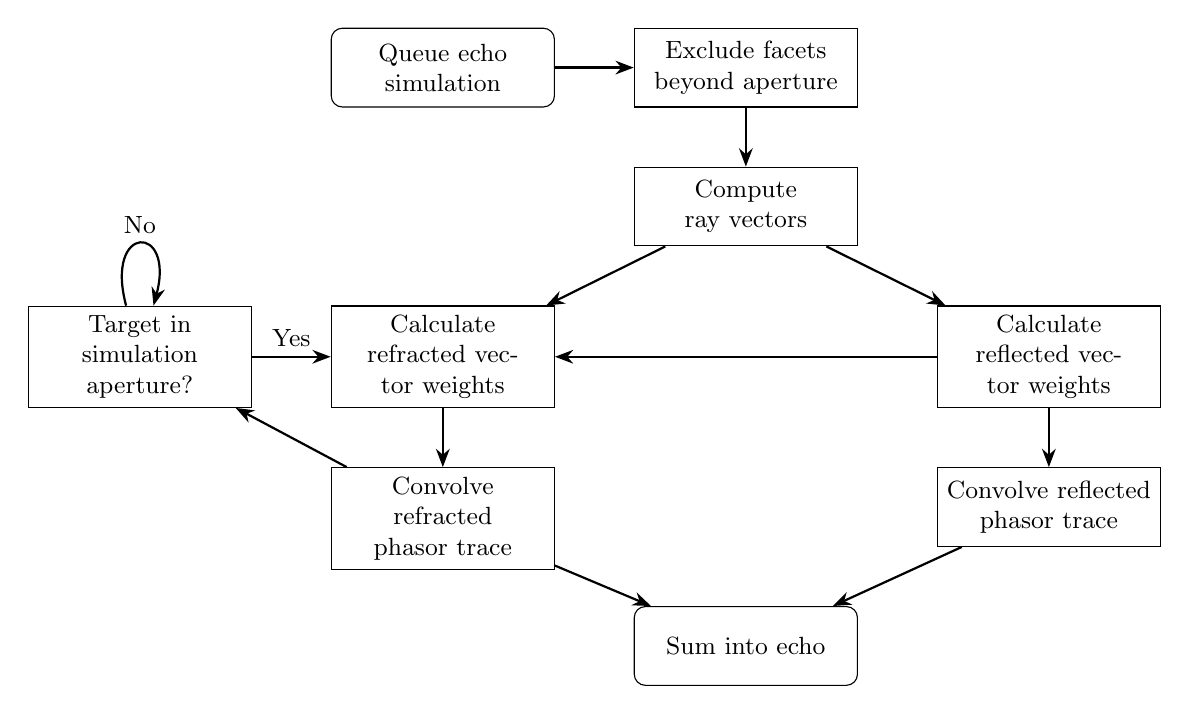
\begin{tikzpicture}[
    node distance=0.75cm and 1.0cm,
    every node/.style={font=\small},
    startstop/.style={
        rectangle,
        rounded corners,
        text width=2.6cm,
        minimum height=1cm,
        text centered,
        draw=black
    },
    process/.style={
        rectangle,
        text width=2.6cm,
        minimum height=1cm,
        text centered,
        draw=black
    },
    arrow/.style={
        thick,
        -{Stealth}
    }
]

% --- input nodes ---
\node (start) [startstop] {Queue echo simulation};

% --- proc nodes ---
\node (init) [process, right=of start] {Exclude facets beyond aperture};
\node (computegeom) [process, below=of init] {Compute ray vectors};
\node (reflenergy) [process, below right=of computegeom] {Calculate reflected vector weights};
\node (refrenergy) [process, below left=of computegeom] {Calculate refracted vector weights};
\node (reflconv) [process, below=of reflenergy] {Convolve reflected phasor trace};
\node (refrconv) [process, below=of refrenergy] {Convolve refracted phasor trace};
\node (targapt) [process, left=of refrenergy] {Target in simulation aperture?};

% --- output nodes ---
\node (sumtrace) [startstop, below left=of reflconv] {Sum into echo};

% --- arrows ---
\draw [arrow] (start) -- (init);
\draw [arrow] (init) -- (computegeom);
\draw [arrow] (computegeom) -- (reflenergy);
\draw [arrow] (computegeom) -- (refrenergy);
\draw [arrow] (reflenergy) -- (refrenergy);
\draw [arrow] (reflenergy) -- (reflconv);
\draw [arrow] (refrenergy) -- (refrconv);
\draw [arrow] (reflconv) -- (sumtrace);
\draw [arrow] (refrconv) -- (sumtrace);
\draw [arrow] (targapt) -- node[midway, above]{Yes} (refrenergy);
\draw [arrow] (targapt) to[loop above] node{No} ();
\draw [arrow] (refrconv) -- (targapt); 

\end{tikzpicture}
\caption{Flow chart for the simulation of a single echo within a radargram.}
\label{fig:flowchart}
\end{figure*}

\section{Performance Comparison}
This section might be a bad idea, given the whole point target versus layer conundrum. Not necessarily validation, but comparison to other simulators?

\section{Examples}

\subsection{Flat Layer}

\begin{enumerate}
    \item Point target under flat surface with flat layer beneath it. 
    \item This is composed of many targets
    \item We have some attenuation geometry (window?)
    \item Everything focuses
    \item Good news it all works properly! (focuses, is the dB for a single point correct?)
\end{enumerate}

\subsection{Convolution vs Non-convolution}

\subsection{Korolev Crater}
\begin{itemize}
    \item We turned the MOLA topography, combined with the mars aeroid to generate the faceted surface \cite{smith_mars_2001}.
    \item We used sharad parameters and orbital information to get the spacecraft transit
    \item We used the subsurface layers identified in \cite{brothers_threedimensional_2016} as our point targets
    \item We interpolated and widened the layers to improve detection
    \item We focused the data using range doppler. 
    \item It matches the data well. 
    \item Show raw, focused, subsurface cross section, and layers figures.
\end{itemize}

\subsection{NPLD}

\subsection{Thwaites Glacier?}
First from Dusty's paper [in review]
\begin{equation}
    \frac{2\pi^2R}{\lambda} > \mathrm{SNR_{max}}
\end{equation}
Using something such as \cite{kaundinya_multi-channel_2024} which operates at 900 MHz and an altitude of 5 us (750 m) yields:
\begin{equation}
    \frac{2\pi^2\cdot750}{0.33}=44861\rightarrow10\log(44861)=46\mathrm{dB}
\end{equation}


\section{Other applications / Notes?}
\begin{itemize}
    \item Can be used for ionosphere raytracing!
    \item Architecture can be modified for a bistatic setup.
\end{itemize}


\section{Conclusion}
The conclusion goes here.


\section*{Acknowledgments}
This should be a simple paragraph before the References to thank those individuals and institutions who have supported your work on this article.



{\appendix[Proof of the Zonklar Equations]
Use $\backslash${\tt{appendix}} if you have a single appendix:
Do not use $\backslash${\tt{section}} anymore after $\backslash${\tt{appendix}}, only $\backslash${\tt{section*}}.
If you have multiple appendixes use $\backslash${\tt{appendices}} then use $\backslash${\tt{section}} to start each appendix.
You must declare a $\backslash${\tt{section}} before using any $\backslash${\tt{subsection}} or using $\backslash${\tt{label}} ($\backslash${\tt{appendices}} by itself
 starts a section numbered zero.)}



%{\appendices
%\section*{Proof of the First Zonklar Equation}
%Appendix one text goes here.
% You can choose not to have a title for an appendix if you want by leaving the argument blank
%\section*{Proof of the Second Zonklar Equation}
%Appendix two text goes here.}

\printbibliography


\newpage

\section{Biography Section}
If you have an EPS/PDF photo (graphicx package needed), extra braces are
 needed around the contents of the optional argument to biography to prevent
 the LaTeX parser from getting confused when it sees the complicated
 $\backslash${\tt{includegraphics}} command within an optional argument. (You can create
 your own custom macro containing the $\backslash${\tt{includegraphics}} command to make things
 simpler here.)
 
\vspace{11pt}

\bf{If you include a photo:}\vspace{-33pt}
\begin{IEEEbiography}[{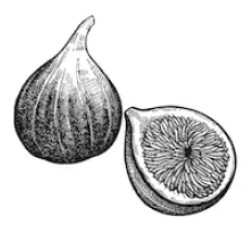
\includegraphics[width=1in,height=1.25in,clip,keepaspectratio]{fig1}}]{Michael Shell}
Use $\backslash${\tt{begin\{IEEEbiography\}}} and then for the 1st argument use $\backslash${\tt{includegraphics}} to declare and link the author photo.
Use the author name as the 3rd argument followed by the biography text.
\end{IEEEbiography}

\vspace{11pt}

\bf{If you will not include a photo:}\vspace{-33pt}
\begin{IEEEbiographynophoto}{John Doe}
Use $\backslash${\tt{begin\{IEEEbiographynophoto\}}} and the author name as the argument followed by the biography text.
\end{IEEEbiographynophoto}




\vfill

\end{document}


